\documentclass[a4paper, 14pt]{extarticle}
% Imports
\usepackage[T2A]{fontenc}
\usepackage[utf8]{inputenc}
\usepackage[russian]{babel} 
\usepackage{graphicx}
\usepackage{hyphenat}
\usepackage{geometry}
\usepackage{hyperref}
\usepackage{float}

\graphicspath{ {../pics/} }

\geometry
{
	a4paper,
	total={170mm,257mm},
	left=20mm,
	top=20mm,
}

\begin{document}
\begin{flushright}
	Козлов Д.В.\\М01-104а	
\end{flushright}


\section*{Построение BER кривых для QAM модуляции}
 
В этой работе был реализован генератор произвольного
квадратного M-QAM (где М -- степень числа 4) созвездия
с кодировкой Грея.

Произведено сравнение теоритических зависимостей
BER от $E_b/N_0$ с результатами симуляции.
Теоритические формулы BER, которые были
использованы в этой работе, приведены
\href{https://www.mathworks.com/help/comm/ug/
analytical-expressions-used-in-berawgn-function
-and-bit-error-rate-analysis-app.html}{\underline{здесь}}.

На рисунках \ref{fig:qam4} - \ref{fig:qam4096} приведены
результаты симуляции. Из графиков видно, что теоритические
кривые совпадают с результатами симуляции.

\begin{figure}[h]
    \centering
    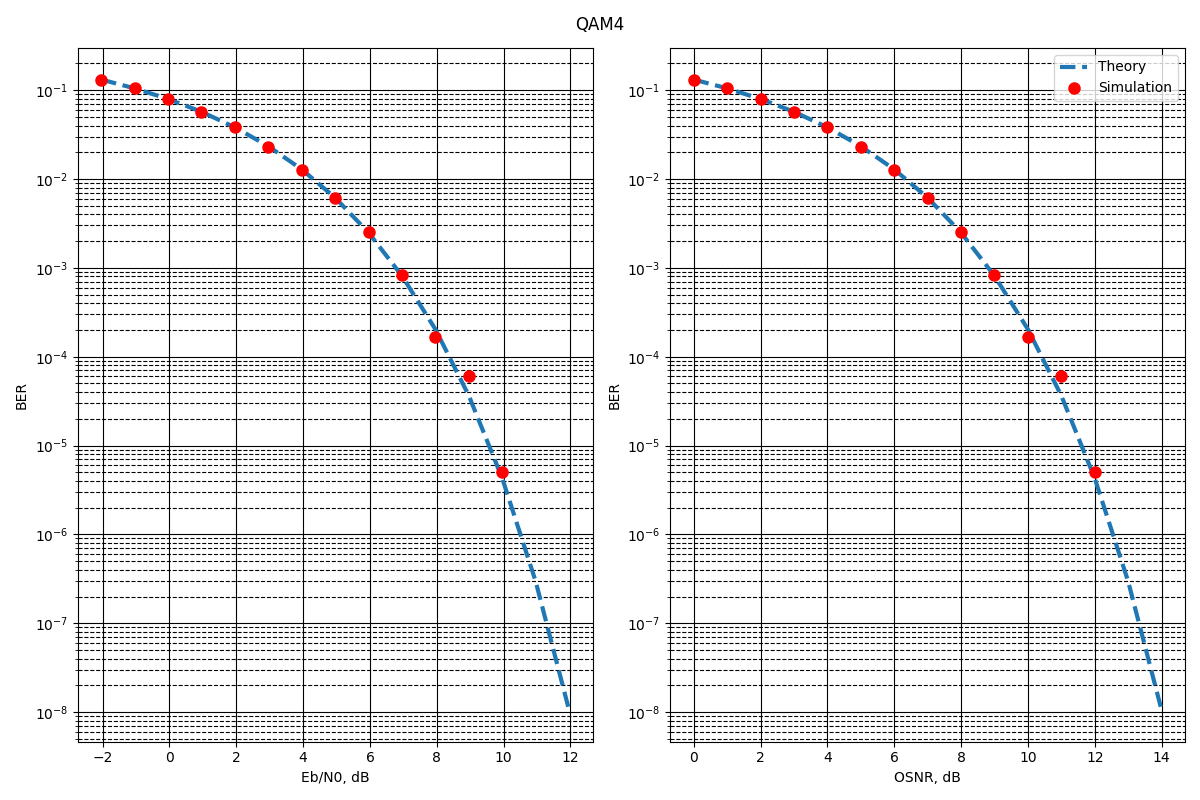
\includegraphics[width=1\textwidth]{QAM4.png}
    \caption{Результат симуляции для QAM4}
    \label{fig:qam4}
\end{figure}
\begin{figure}[]
	\centering
    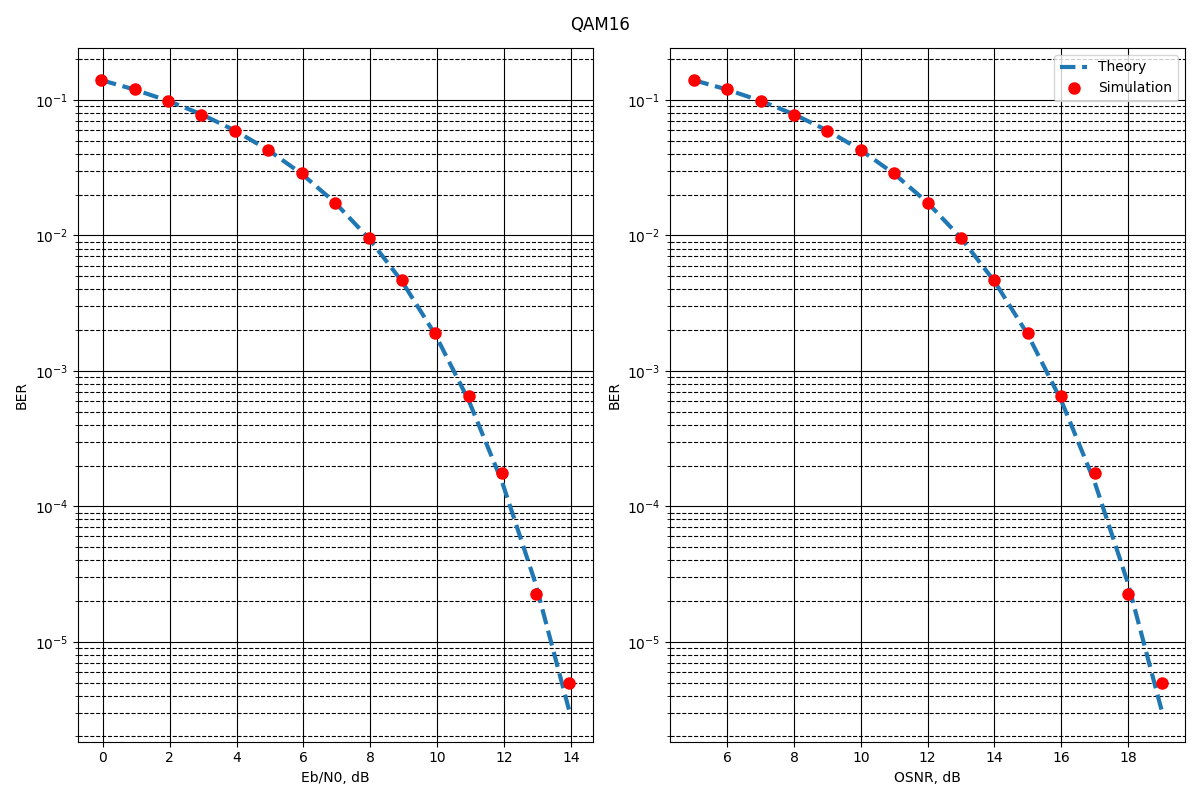
\includegraphics[width=1\textwidth]{QAM16.png}
    \caption{Результат симуляции для QAM16}
    \label{fig:qam16}
	\centering
    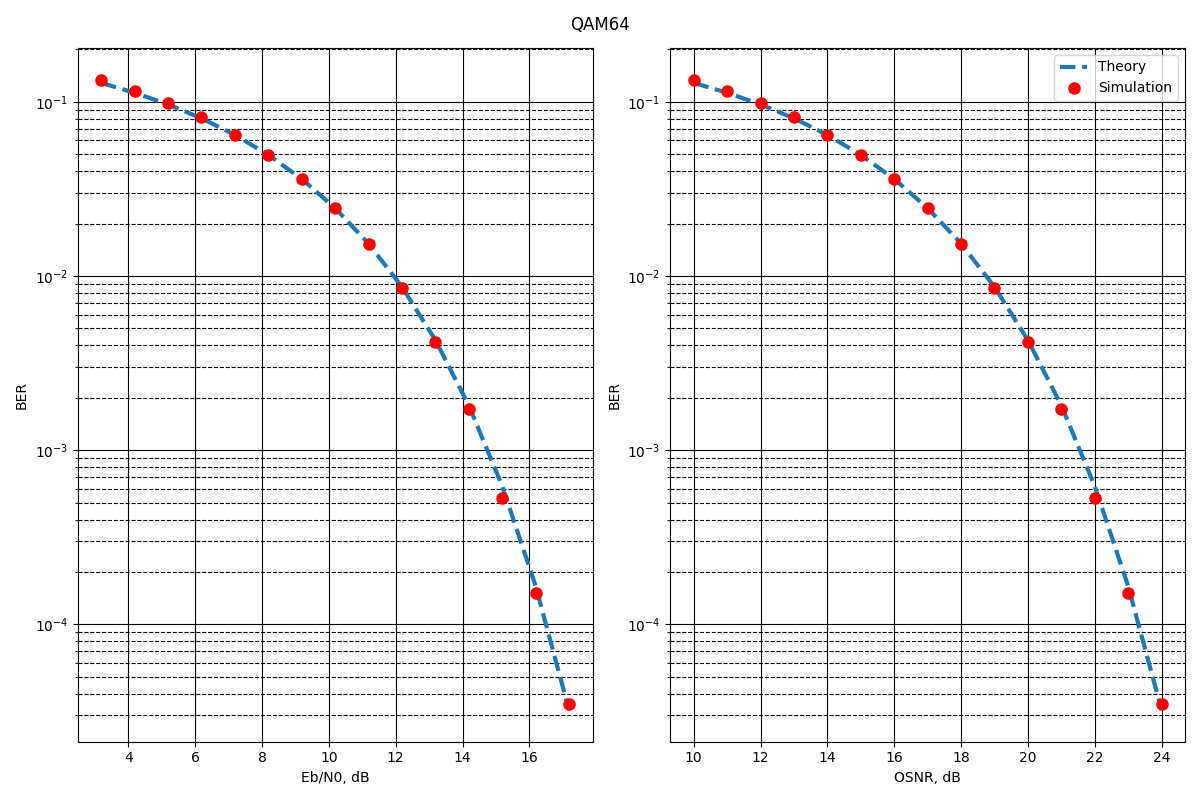
\includegraphics[width=1\textwidth]{QAM64.png}
    \caption{Результат симуляции для QAM64}
    \label{fig:qam64}
\end{figure}
\begin{figure}[]
	\centering
    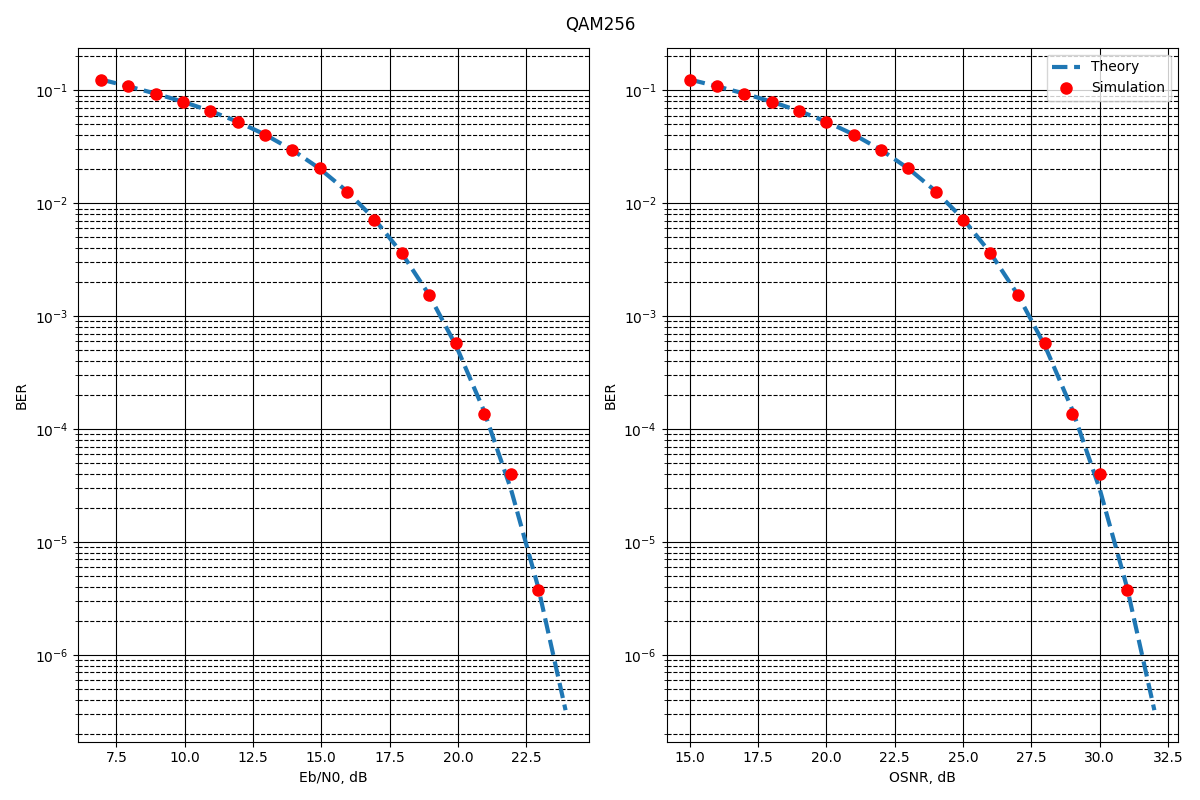
\includegraphics[width=1\textwidth]{QAM256.png}
    \caption{Результат симуляции для QAM256}
    \label{fig:qam256}
	\centering
    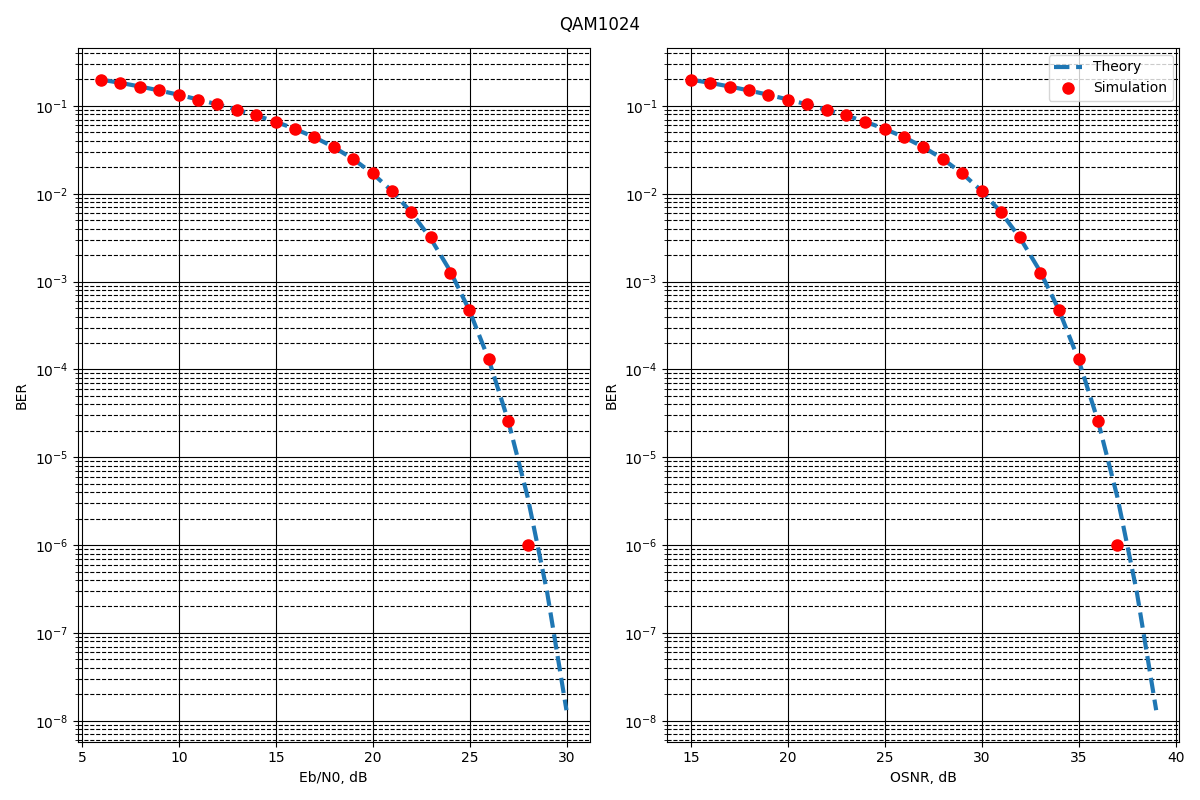
\includegraphics[width=1\textwidth]{QAM1024.png}
    \caption{Результат симуляции для QAM1024}
    \label{fig:qam1024}
\end{figure}
\begin{figure}[]
	\centering
    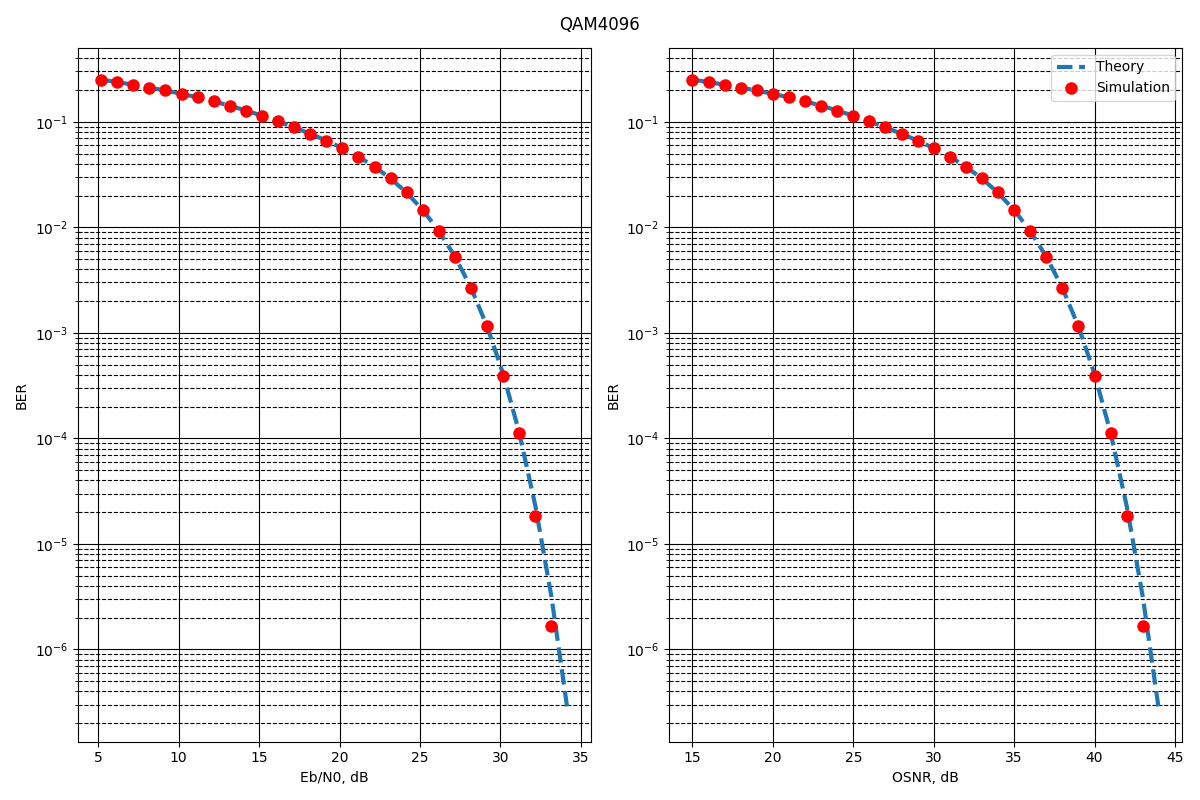
\includegraphics[width=1\textwidth]{QAM4096.png}
    \caption{Результат симуляции для QAM4096}
    \label{fig:qam4096}
\end{figure}


\end{document}
